\section{Introduction}
Mobile systems have clear requirements for user satisfaction: they
must meet performance goals necessary for interacting with sensors and
human users and must conserve energy to maximize battery life.  To
address these conflicting requirements, mobile processors have become
increasingly diverse, exposing diverse heterogeneous resources that
must be managed by software. Meeting performance requirements is
further complicated by the dynamic nature of computing systems:
application resource demands can vary widely as a function of input or
application phase and multiple applications may compete for resources.

\begin{figure}
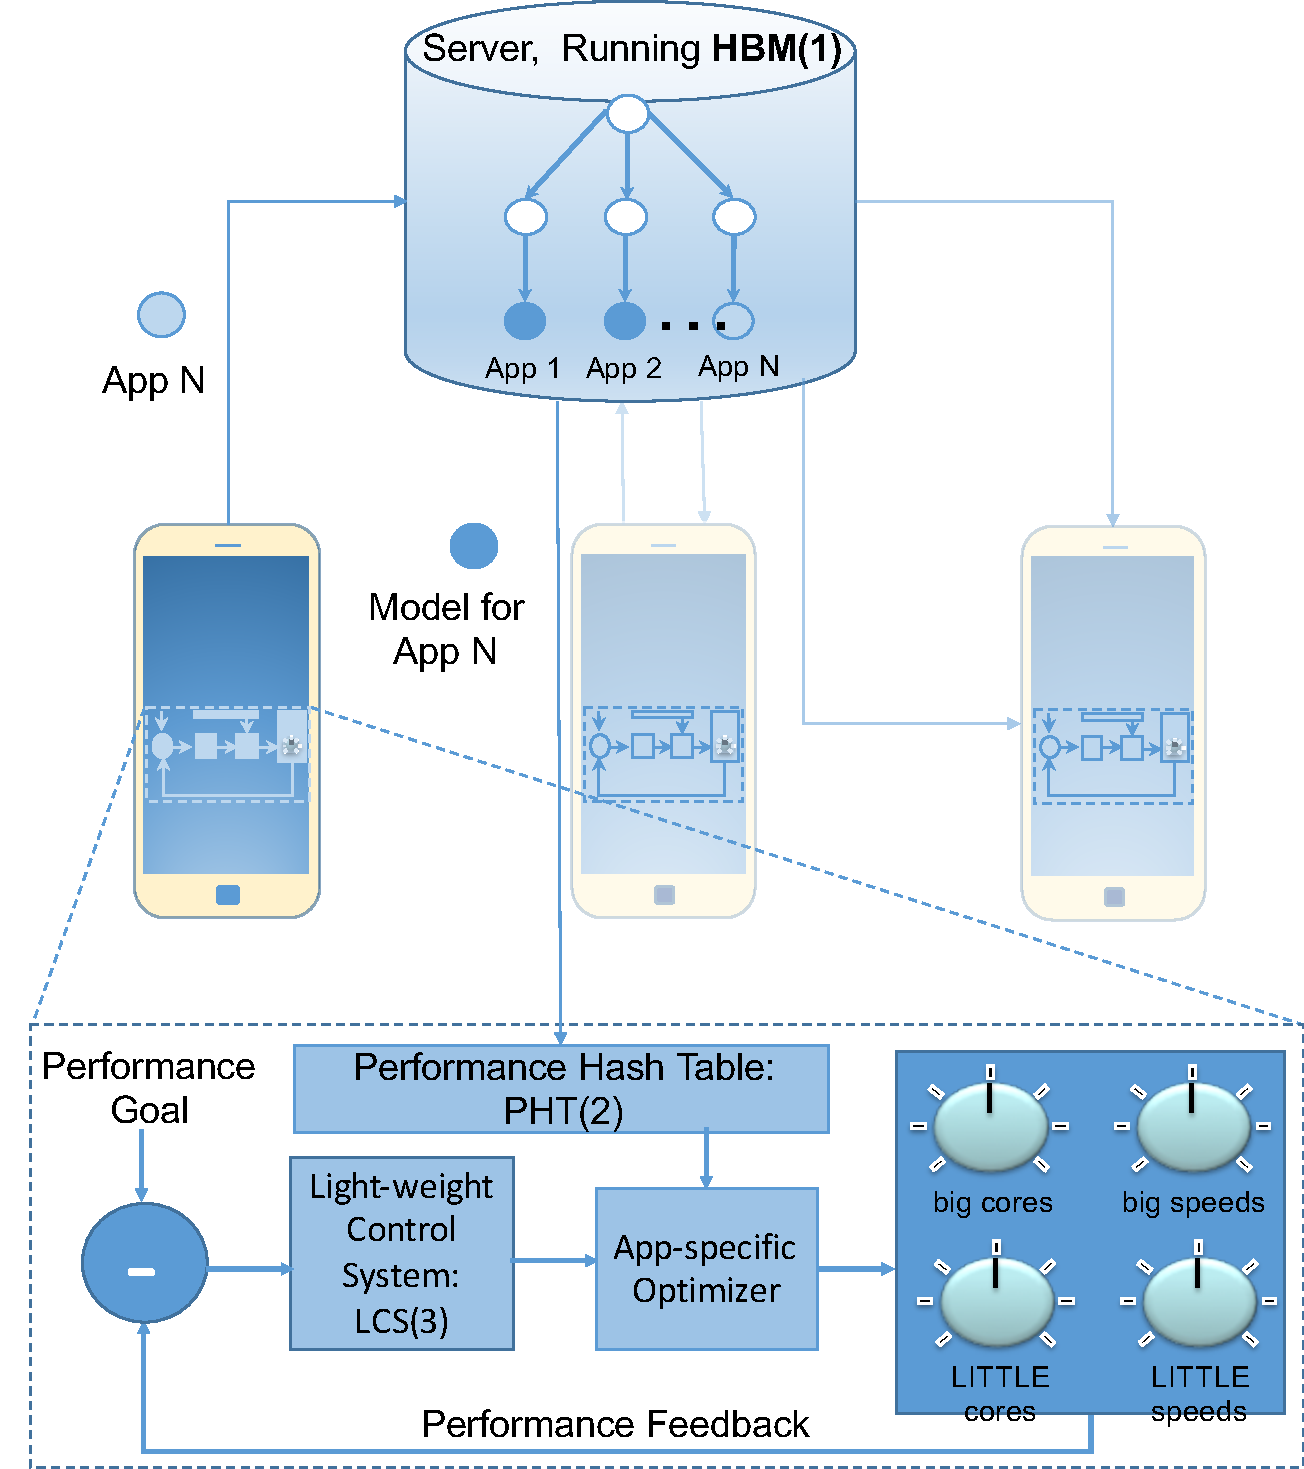
\includegraphics[width=\columnwidth]{figures/mobile-leo-poet.pdf}
\caption{\SYSTEM{} overview.}
  \label{fig:overview}
\end{figure}

Thus, two challenges arise to meeting performance requirements with
minimal energy on mobile systems: (1) complexity and (2) dynamics.
Machine learning approaches handle the complex power/performance
tradeoff spaces that arise on heterogeneous mobile systems
\cite{reddiHPCA2013,dubach2010,Bitirgen2008,Ipek,Koala,LEO,Flicker,Ponamarev},
but they have no established mechanisms for reacting to environmental
fluctuations.  \PUNT{Such approaches can learn complex models,
  identifying and avoiding local extrema that lead to inefficient
  resource usage.}  Control theoretic techniques explicitly address
system and resource dynamics
\cite{Hellerstein2004a,Chen2011,PTRADE,POET,ControlWare,Agilos,grace2},
but rely on linear models that do not capture the diversity of modern
hardware.  \PUNT{Control techniques provide a formal basis for
  reasoning about dynamics and are robust to application, input, and
  workload fluctuations. These approaches have complementary strengths
  and weaknesses.  Learning handle complexity but have no established
  mechanism for managing system dynamics.  Control approaches handle
  dynamics but rely on linear models that do not capture the diversity
  of modern hardware. } Individually, neither control nor learning
meet the challenges of modern mobile resource management.

We therefore propose \SYSTEM{}\footnote{\textbf{C}ontrol \textbf{A}nd
  \textbf{L}earning for \textbf{O}ptimal \textbf{R}esource
  \textbf{E}nergy \textbf{E}fficiency}, a combination of learning and
control consisting of the three components shown in
\figref{fig:overview}: (1) a hierarchical Bayesian model (HBM) that
learns application-specific relationships between performance/power
and resource usage, (2) a lightweight control system (LCS) that
dynamically tunes resource usage to meet performance requirements with
minimal energy, and (3) a performance hash table (PHT), which is the
interface between learning and control.  \SYSTEM{}'s design has two
unique features:
\begin{itemize}
\item \textit{Remote Learning:} Sophisticated learning techniques
  produce accurate models of complicated systems but they are
  computationally expensive.  \SYSTEM{} mitigates this expense by
  running the learner on a remote server. This approach not only
  addresses overhead, it allows the learner to aggregate data from
  multiple devices, improving learning accuracy.
\item \textit{Fast Control:} The controller must not significantly
  impact performance or energy on the mobile device.  Yet, the
  controller must solve a constrained optimization problem to meet the
  performance goal with minimal energy.  To overcome this difficulty,
  \SYSTEM{}'s remote learner constructs a PHT for each application.
  While building the PHT is expensive, it allows the LCS to solve the
  constrained optimization problem in constant ($O(1)$) time.
\end{itemize}
The PHT is \SYSTEM{}'s key enabler.  It is the interface between the
HBM and LCS, allows the HBM to be executed remotely, and enables fast
mobile optimization.


\PUNT{
\SYSTEM{} overcomes three difficulties of combining learning and
control:
\begin{itemize}
\item \textit{Model differences:} The learner produces non-linear
  models of discrete resources, while the control system is based on
  continuous, linear models.  \SYSTEM{} addresses this challenges by
  scheduling resources in time to map a continuous control into
  discrete resource configurations.
\item \textit{Learning overhead:} Sophisticated learning techniques
  produce accurate models of complicated systems but they are
  computationally expensive.  \SYSTEM{} overcomes this difficulty by
  running the learner on a remote server. This approach not only
  addresses overhead, it allows the learner to aggregate data from
  multiple devices, improving learning accuracy.
\item \textit{Control overhead:} The controller must not significantly
  impact performance or energy on the local device.  Therefore,
  \SYSTEM{} stores the learned models in the PHT, which allows it to
  schedule resources in constant ($O(1)$) time.  
\end{itemize}
The PHT is \SYSTEM{}'s key enabler.  It serves as the interface
between the HBM and LCS, allows the learner to be executed remotely,
and enables fast scheduling on the local device.
}
\PUNT{
The main challenge in combining a learning system with a control system is that the learner produces non-linear models of
resources (\eg cores and clockspeeds) which are discrete, while the control
system is based on continuous linear models.  \SYSTEM{} bridges this
gap by scheduling resources in time to meet a performance requirement
with minimal energy.  

The second challenge is that our learner (HBM) produces accurate
models of power and performance, but like many sophisticated machine learning based models it is computationally expensive,
so in \SYSTEM{} the HBM runs on a remote server.  Moreover, as it is remote, it
is also capable of aggregating data from multiple devices, which makes learner more powerful. The controller (LCS) runs on individual mobile devices and receives models from the HBM.

Thirdly, for great user satisfaction, we would like this system to be fast. Hence, we propose that  these models are stored in the PHT, a data structure that allows the LCS to determine energy minimal resource schedules in constant time. The PHT is \SYSTEM{}'s key enabler.  While learning and control
systems exist, their combination requires an appropriate interface.
 %The PHT stores the learned models in such a way that this optimization problem can be solved in constant time, making it appropriate for use on a mobile device.   
 While only tested with \SYSTEM{} we believe the PHT is general enough to be used by different learning and control systems, or even to solve different optimization problems.
}


% While control and learning frameworks exist, the key to combining them
% is creating an interface between the learning and control systems.
% Specifically, learning frameworks for resource management map
% configurations (\eg{} resource allocations) into estimated performance
% and power.  These mappings are discrete and non-linear, capturing the
% behavior of the underlying system.  Controllers, in contrast, work
% with continuous linear models.  Therefore, our proposed combination of
% learning and control requires an interface to convert the discrete
% non-linear learned models into continuous linear models.  We address
% this challenge by forming the lower convex hull of points on the
% learned power/performance tradeoff space.  Interpolating between these
% points gives us a piecewise linear function that is appropriate for
% control models, yet still captures the significant behavior of the
% underlying system.  This interface allows us to combine the approaches
% studied in this paper, and we believe it is sufficiently general to
% apply to other combinations of learning and control as well.
\PUNT{ We test \SYSTEM{} on ARM big.LITTLE platforms with 20 different
  benchmarks to evaluate the HBM's ability to learn application
  specific models and the LCS's ability to deliver performance
  efficiently.  We compare to published learning and control methods
  in a variety of settings.  While many applications have inherent
  dynamics (\ie{}{} different processing phases), we explicitly test
  the ability to adapt to the unknown by running each application with
  other, random applications.} 

This paper makes the following contributions:
\begin{itemize}
\item The combination of a hierarchical Bayesian learning with a
  lightweight control system to deliver performance with minimal
  energy on mobile systems.
\item An interface for combining learned models of discrete resource
  usage with continuous control models of resource dynamics.
\item Comparison to independent learning and control techniques to
  evaluate performance and energy.
\end{itemize}

We implement the HBM on an x86 server and the LCS for ARM big.LITTLE
devices and evaluate across 20 benchmarks.  We find that \SYSTEM{}:
\begin{itemize}
\item \textbf{Delivers Reliable Performance: } We calculate the error
  between the desired and delivered performance.  When running one
  application at a time, \SYSTEM{} achieves an average error of 2.1\%,
  compared to 3.4-5.4\% for existing learning methods and 4.6\% for
  existing control approaches.
\item \textbf{Uses Lower Average Energy:} When running one application
  at a time, \SYSTEM{} achieves an average energy consumption of 7\%,
  greater than optimal compared to 25-52\% for existing learning
  methods and 26\% for existing control approaches.
\item \textbf{Provides Better Worst Case Behavior:} In the single
  application case, \SYSTEM{} worst observed error across all
  applications and targets is 9\% compared to 19-73\% for prior
  learning methods and 25\% for existing control methods.  The worst
  observed energy for \SYSTEM{} is 1.82$\times$ greater than optimal,
  while it is 4-12$\times$ greater for learning and 2.9 $\times$
  greater for control.
\item \textbf{Adapts to Dynamics:} We test \SYSTEM{}'s ability to deal
  with changing environments by running each benchmark with a
  performance target and then randomly starting another application on
  one core.  Even though the available resources fluctuate
  dynamically, \SYSTEM{}'s worst performance error is 30\%, while it
  is 71-84\% for prior learning approaches and 35\% for prior control
  approaches.
\end{itemize}
